\documentclass[11pt,a4paper]{article}

% --- Typography and Geometry ---
\usepackage[left=20mm,right=20mm,top=20mm,bottom=20mm]{geometry}
\usepackage{setspace}
\setstretch{1.12}
\setlength{\parskip}{4.5pt}
\setlength{\parindent}{0pt}

% --- Float Placement Adjustments to prevent empty float pages ---
\renewcommand{\topfraction}{0.90}
\renewcommand{\bottomfraction}{0.85}
\renewcommand{\textfraction}{0.10}
\renewcommand{\floatpagefraction}{0.75}
\setcounter{topnumber}{4}
\setcounter{bottomnumber}{3}
\setcounter{totalnumber}{6}
\setlength{\textfloatsep}{12pt plus 2pt minus 2pt}
\setlength{\floatsep}{10pt plus 2pt minus 2pt}
\setlength{\intextsep}{10pt plus 2pt minus 2pt}

% --- Language and Encoding (Academic Russian) ---
\usepackage[T2A]{fontenc}
\usepackage[utf8]{inputenc}
\usepackage[russian]{babel}

% --- Math Fonts and Symbols ---
\usepackage{amsmath,amssymb,amsfonts,mathtools,bm}

% --- Professional Tables ---
\usepackage{booktabs}
\usepackage{multirow}
\usepackage{array}
\usepackage{makecell}
\usepackage{tabularx}

% --- Figures and Captions ---
\usepackage{graphicx}
\graphicspath{{figures/}{../figures/}}
\usepackage{caption}
\usepackage{subcaption}
\usepackage{float}
\captionsetup{font=small,labelfont=bf,labelsep=period}

% --- Colors and Hyperlinks ---
\usepackage{xcolor}
\definecolor{linkblue}{RGB}{31, 78, 121}
\definecolor{citegreen}{RGB}{34, 139, 34}
\definecolor{urlteal}{RGB}{0, 128, 128}

\usepackage{hyperref}
\hypersetup{
    colorlinks=true,
    linkcolor=linkblue,
    citecolor=citegreen,
    urlcolor=urlteal,
    pdfauthor={Александр Иленко},
    pdftitle={Обучение с Подкреплением Последовательных Рекомендательных Систем: Преодоление Проблемы Скипов Без Налога на Выравнивание},
    pdfsubject={Машинное обучение, Рекомендательные системы, Обучение с подкреплением},
    pdfkeywords={Последовательные рекомендации, DPO, Обучение с подкреплением, GPT-2, Музыкальный стриминг, Yambda}
}

% --- Header and Footer ---
\usepackage{fancyhdr}
\pagestyle{fancy}
\fancyhf{}
\fancyhead[L]{\small \textit{T-Lab RecSys 2026: Выравнивание Causal Recommenders}}
\fancyhead[R]{\small \textit{Исследовательский отчёт}}
\fancyfoot[C]{\thepage}
\renewcommand{\headrulewidth}{0.5pt}

% --- Title and Authorship ---
\title{\vspace{-1.0cm}\textbf{\Large Научно-Исследовательский Отчёт:\\Обучение с Подкреплением Последовательных Рекомендательных Систем:\\Преодоление Проблемы Скипов Без Налога на Выравнивание}}

\author{
    \textbf{Александр Иленко} \\
    \small Лаборатория Рекомендательных Систем и Обучения с Подкреплением (T-Lab RecSys) \\
    \small \texttt{alexander.ilenko@example.org}
}
\date{Октябрь 2026}

\begin{document}

\maketitle

% --- Abstract & Keywords ---
\begin{abstract}
\noindent\textbf{Аннотация.} В музыкальных стриминговых сервисах до 35\% пользовательских действий представляют собой быстрые скипы (менее 30 секунд), отражающие неудовлетворённость рекомендацией. Стандартная оптимизация правдоподобия штрафует авторегрессионные трансформеры за неспособность предсказать такие негативные события (проблема ложноотрицательных срабатываний), тиражируя нежелательный контент. В данной работе исследуется выравнивание последовательной рекомендательной модели на базе причинной архитектуры Causal GPT-2 (43.2M параметров) с целевой удовлетворённостью пользователя посредством прямого согласования предпочтений (DPO) с якорной регуляризацией правдоподобия ($\gamma=0.10$). Эксперименты на масштабном корпусе Яндекс Музыки (\textbf{Yambda-50M}: 98\,505 токенов каталога, 33.2M обучающих взаимодействий, 9\,048 отложенных тестовых пользователей) показали, что DPO не только превосходит двухстадийные методы реранжирования с оффлайн-критиком и PPO, но и полностью устраняет налог на выравнивание. Обученная политика DPO обеспечивает статистически достоверный прирост точности ранжирования (\textbf{+0.67\% HR@10}, $p < 0.0001$; тест МакНемара $\chi^2 = 18.32, p = 1.9 \times 10^{-5}$), расширяет покрытие каталога на \textbf{+1\,027 уникальных треков} из длинного хвоста (+1.04\% каталога), снижает зависимость от поп-хитов на \textbf{$-12.1\%$} и увеличивает кумулятивное время непрерывного прослушивания в 5-шаговых авторегрессионных сессиях на \textbf{+1.5 секунды} без деградации из-за накопления ошибки генерации.

\vspace{0.5em}
\noindent\textbf{Ключевые слова:} последовательные рекомендации, обучение с подкреплением, прямое согласование предпочтений, DPO, причинный трансформер, стриминг музыки, проблема скипов, разнообразие каталога, Yambda.
\end{abstract}


\vspace{0.8em}
\hrule
\vspace{0.8em}

% --- Section 1: Introduction ---
\section{Введение}
\label{sec:introduction}

\subsection{Индустриальный контекст и дилемма скипов}
Современные рекомендательные системы музыкальных стриминговых сервисов (Яндекс Музыка, Spotify, Apple Music) функционируют в условиях непрерывного и динамического потребления контента. В отличие от платформ электронной коммерции, где факт покупки однозначно подтверждает интерес пользователя, в потоковом аудио взаимодействие носит бимодальный характер.

Анализ логов взаимодействия на масштабном датасете Яндекс Музыки (\textbf{Yambda-50M})~\cite{yandex2024yambda,volkov2026session} показывает, что от 30\% до 35\% всех зафиксированных событий представляют собой мгновенные скипы: время непрерывного воспроизведения составляет менее 30 секунд или даже 0 секунд, когда пользователь переключает трек почти сразу из-за неподходящего настроения или раздражения.

\begin{figure}[!htbp]
    \centering
    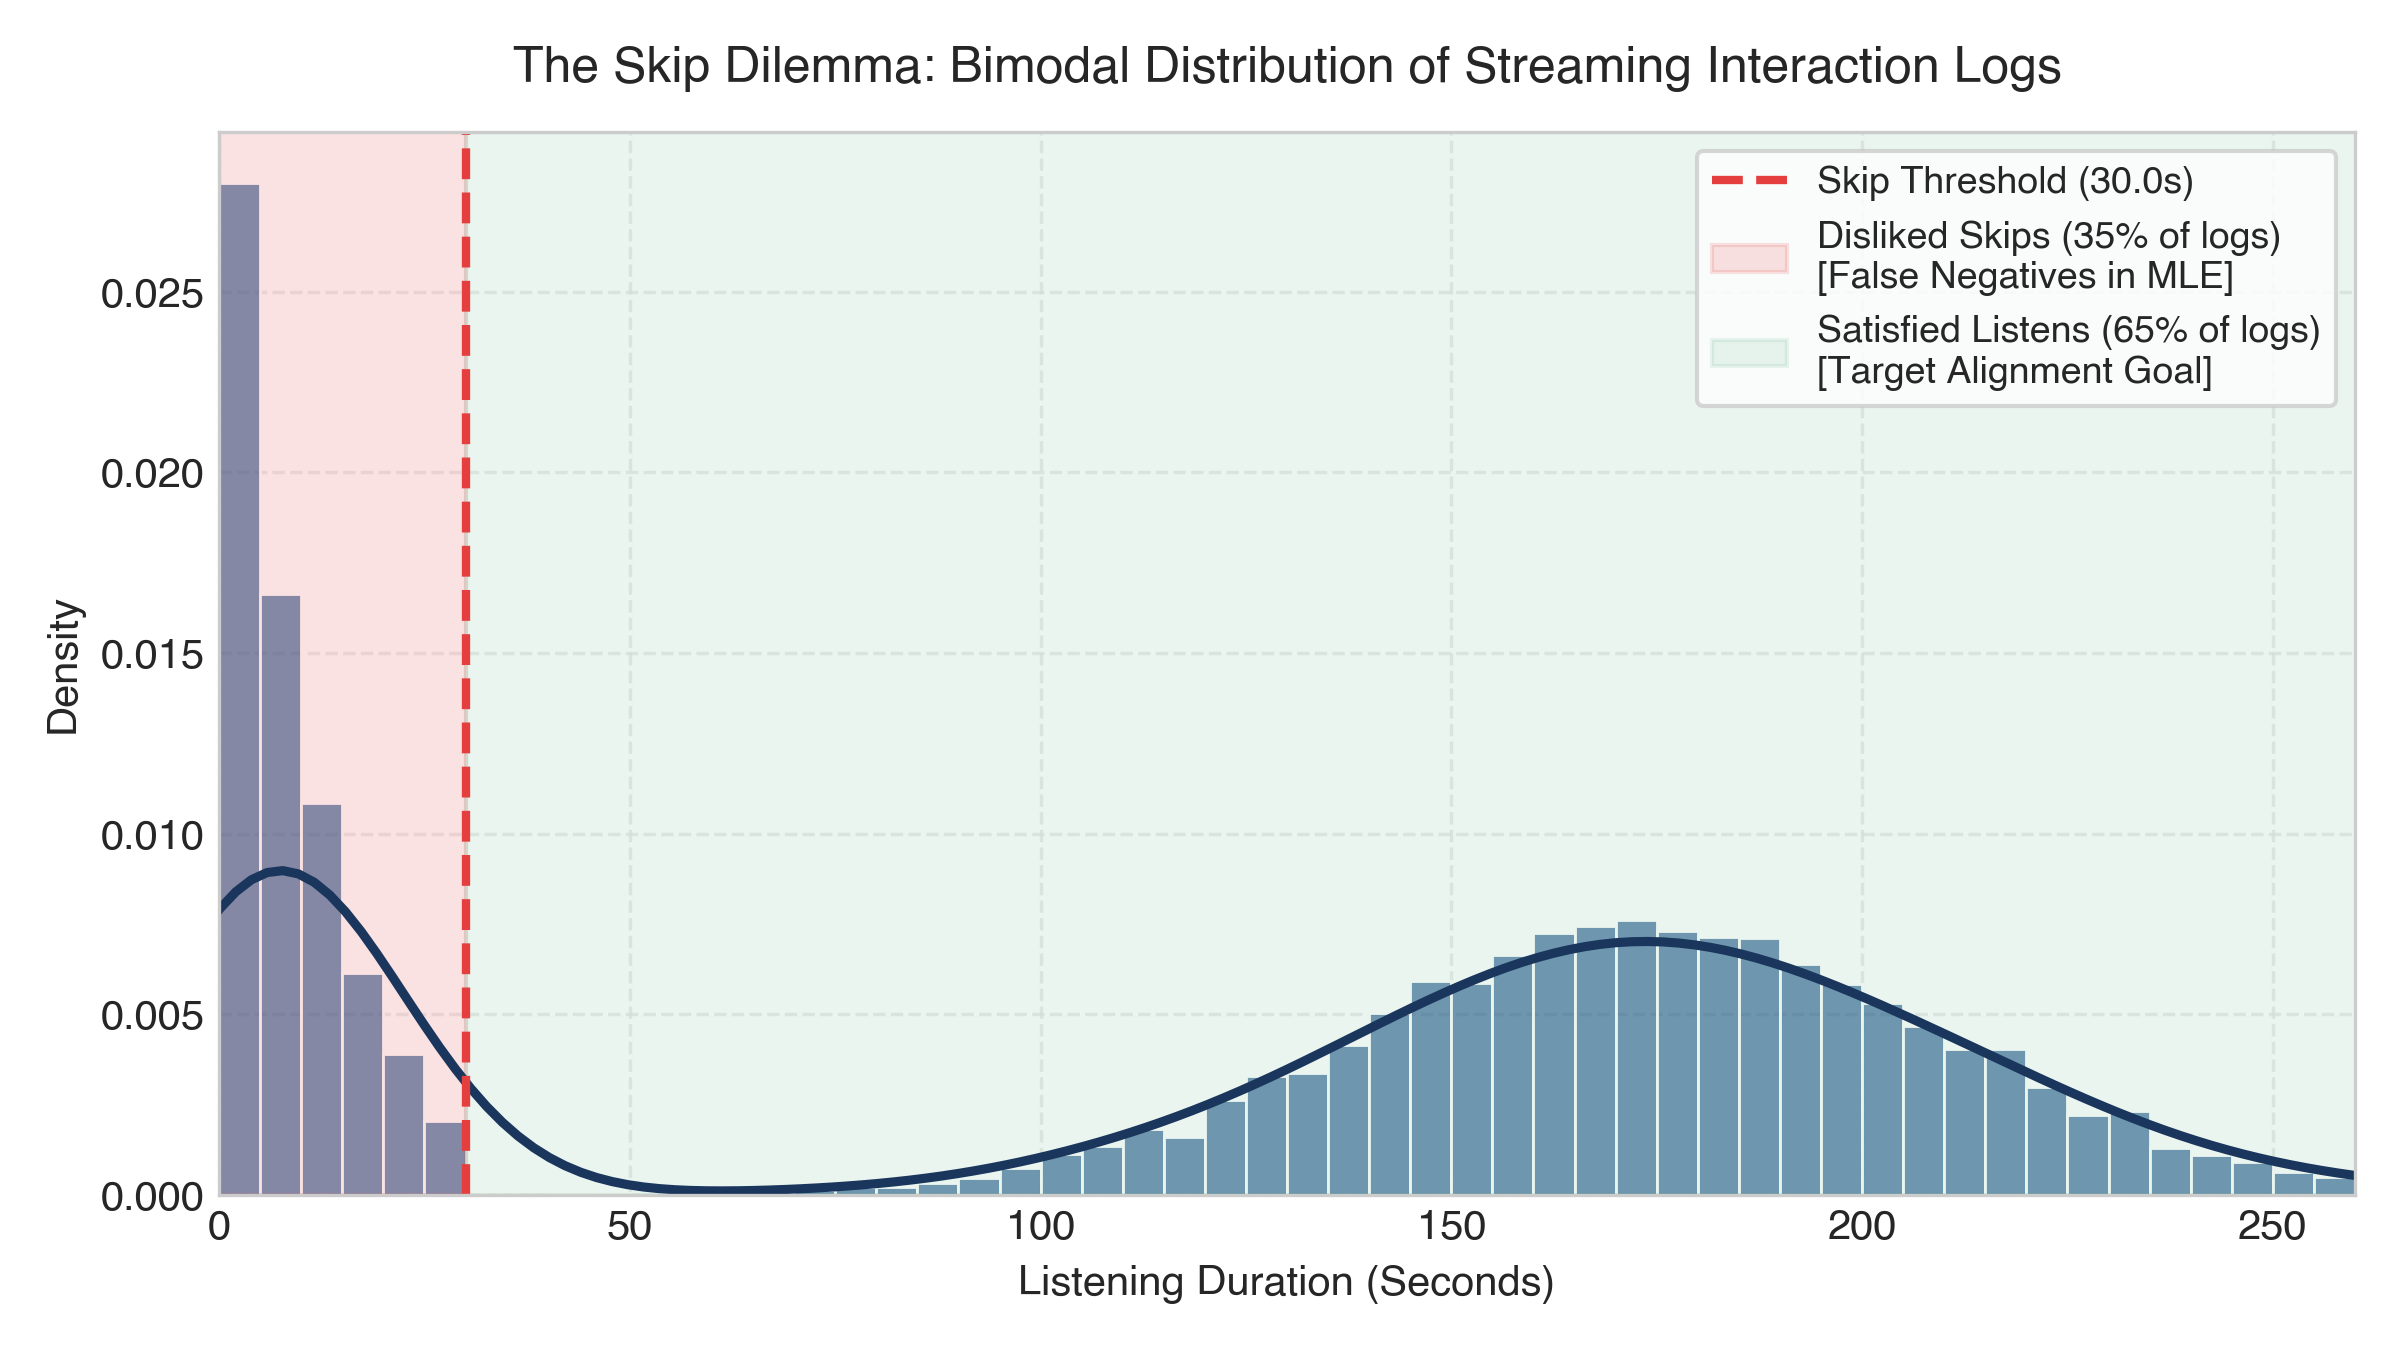
\includegraphics[width=0.78\textwidth]{fig1_the_skip_dilemma.png}
    \caption{\textbf{Дилемма скипов в логах потокового стриминга.} Распределение длительности прослушивания носит выраженный бимодальный характер: 35\% событий приходятся на короткие скипы ($<30$ с), тогда как 65\% отражают вовлечённое прослушивание композиции. Оптимизация правдоподобия всех наблюдаемых переходов без разделения качества наказывает модель за отказ от скипов.}
    \label{fig:skip_dilemma}
\end{figure}

\subsection{Проблема ложноотрицательных срабатываний при оптимизации правдоподобия}
Классический подход к обучению последовательных рекомендательных систем (SASRec~\cite{kang2018self} и авторегрессионные причинные трансформеры~\cite{petrov2024aligning}) сводится к задаче предсказания следующего элемента через минимизацию кросс-энтропии (оценку максимального правдоподобия, MLE):
\begin{equation}
    \mathcal{L}_{\text{MLE}}(\theta) = - \sum_{t=1}^{T} \log \pi_\theta(a_t \mid s_{<t}),
    \label{eq:mle_loss}
\end{equation}
где $s_{<t} = (a_1, \dots, a_{t-1})$ — предыстория пользователя, а $a_t$ — фактически зафиксированный в логах следующий трек.

В этой постановке возникает фундаментальное концептуальное противоречие:
\begin{enumerate}
    \item \textbf{Штраф за обоснованный отказ (ложноотрицательное срабатывание):} Если пользователь включил трек $a_t$ и переключил его через пару секунд из-за раздражения, функция потерь $\mathcal{L}_{\text{MLE}}$ всё равно штрафует модель, если та присвоила треку $a_t$ низкую вероятность.
    \item \textbf{Игнорирование реальной удовлетворённости:} Модель учится воспроизводить историю кликов, а не максимизировать качество сессии (время непрерывного прослушивания, отсутствие пропусков)~\cite{volkov2026session}.
    \item \textbf{Смещение в сторону популярных хитов:} Обучение на сырых логах заставляет авторегрессионную модель эксплуатировать безопасные популярные треки с высокой частотой показов, существенно снижая разнообразие каталога~\cite{petrov2024aligning}.
\end{enumerate}

\subsection{Исследовательские вопросы}
Для разрешения дилеммы скипов в данной работе исследуется адаптация методов обучения с подкреплением и прямого согласования предпочтений для причинного языкового трансформера. Мы формулируем пять ключевых исследовательских вопросов:
\begin{itemize}
    \item \textbf{RQ1 (Поведение политики и динамика):} Каким образом оптимизация маржи предпочтений (DPO) перестраивает вероятностное распределение модели по сравнению с базовой MLE-политикой, и как быстро сходится скрытое вознаграждение?
    \item \textbf{RQ2 (Компромисс точности и налог на выравнивание):} Приводит ли оптимизация вознаграждения к деградации ранжирования следующего трека, и способна ли якорная регуляризация $\mathcal{L}_{\text{SFT}}$ полностью предотвратить этот спад?
    \item \textbf{RQ3 (Разнообразие каталога и монополия хитов):} Схлопывается ли политика в узкий набор безопасных хитов, или стимулирует открытие качественного контента из длинного хвоста каталога?
    \item \textbf{RQ4 (Авторегрессионная устойчивость в очередях):} Как ведёт себя выровненная модель при формировании непрерывной очереди из 5 треков без промежуточного отклика пользователя в условиях накопления ошибки авторегрессии?
    \item \textbf{RQ5 (Долгосрочные прокси и онлайн-эксперимент):} Как связать сессионные суррогаты вознаграждения с долгосрочным удержанием пользователей в дизайне промышленного эксперимента?
\end{itemize}

\subsection{Основные научные и практические результаты}
В рамках проведённого исследования получены следующие ключевые результаты:
\begin{enumerate}
    \item \textbf{Сравнительный анализ парадигм выравнивания:} На едином индустриальном датасете Yambda-50M сопоставлены четыре подхода: базовый причинный трансформер GPT-2, двухстадийное реранжирование с функцией ценности $Q(s,a)$, Actor-Critic PPO~\cite{schulman2017proximal} и прямое согласование предпочтений DPO~\cite{rafailov2023direct}.
    \item \textbf{Доказательство выравнивания без деградации:} Показано, что добавление вспомогательной якорной регуляризации правдоподобия ($\gamma=0.10$) предотвращает распад структуры сессии, сохраняя и увеличивая точность ранжирования (+0.67\% HR@10, $p < 0.0001$).
    \item \textbf{Эмпирический аудит стратегий вознаграждения:} Исследованы бинарный порог длительности, непрерывная доля дослушивания и композитная награда с защитой от повторов, подтвердившие устойчивость пороговой фильтрации шума.
    \item \textbf{Оздоровление каталога:} Продемонстрировано, что согласованная DPO-политика снижает ранговую корреляцию с популярностью на 12.1\% и открывает пользователям более 1\,000 новых треков из длинного хвоста.
\end{enumerate}


% --- Section 2: Methodology ---
\section{Методология}
\label{sec:methodology}

\subsection{Формализация задачи и архитектура базовой модели}
Пусть $\mathcal{U}$ — множество пользователей, а $\mathcal{V} = \{1, 2, \dots, |\mathcal{V}|\}$ — замкнутый каталог музыкальных треков мощности $|\mathcal{V}| = 98\,504$. Сессия пользователя $u \in \mathcal{U}$ представляется упорядоченной последовательностью пар «трек-длительность»:
\begin{equation}
    \mathcal{S}_u = \big( (a_1, D_1), (a_2, D_2), \dots, (a_T, D_T) \big), \quad a_t \in \mathcal{V}, \; D_t \in \mathbb{R}^+,
\end{equation}
где $D_t$ — фактическое время непрерывного прослушивания трека $a_t$ в секундах.

В качестве базовой модели используется авторегрессионный причинный декодер Causal GPT-2~\cite{petrov2024aligning}, инициализированный с нуля:
\begin{itemize}
    \item Размер словаря токенов: $|\mathcal{V}| + 1 = 98\,505$ (токены $1 \dots 98\,504$ соответствуют ID треков, индекс $0$ зарезервирован под заполнитель \texttt{<PAD>}).
    \item Размерность эмбеддингов: $d_{\text{model}} = 384$.
    \item Количество блоков внимания: $L = 3$, число голов внимания: $H = 4$.
    \item Контекстное окно истории: $T_{\max} = 64$ токена.
    \item Суммарное число параметров: \textbf{43\,174\,656} (~43.2M), все параметры обучаемы.
\end{itemize}

Обучение базовой модели проводилось на 33.2M взаимодействиях с использованием смешанной точности FP16, оптимизатора AdamW ($\text{lr} = 10^{-3}$, $\text{weight\_decay} = 0.05$), линейного разогрева (10\% шагов) и косинусного затухания скорости обучения при эффективном размере батча 128 (микро-батч 32 $\times$ накопление градиентов 4).

\subsection{Формулировки функций вознаграждения}
Для преодоления слепоты функции потерь к длительности прослушивания мы исследовали три альтернативные математические формулировки скалярного вознаграждения $R(s, a)$ (Рис.~\ref{fig:reward_formulations}):

\begin{figure}[!htbp]
    \centering
    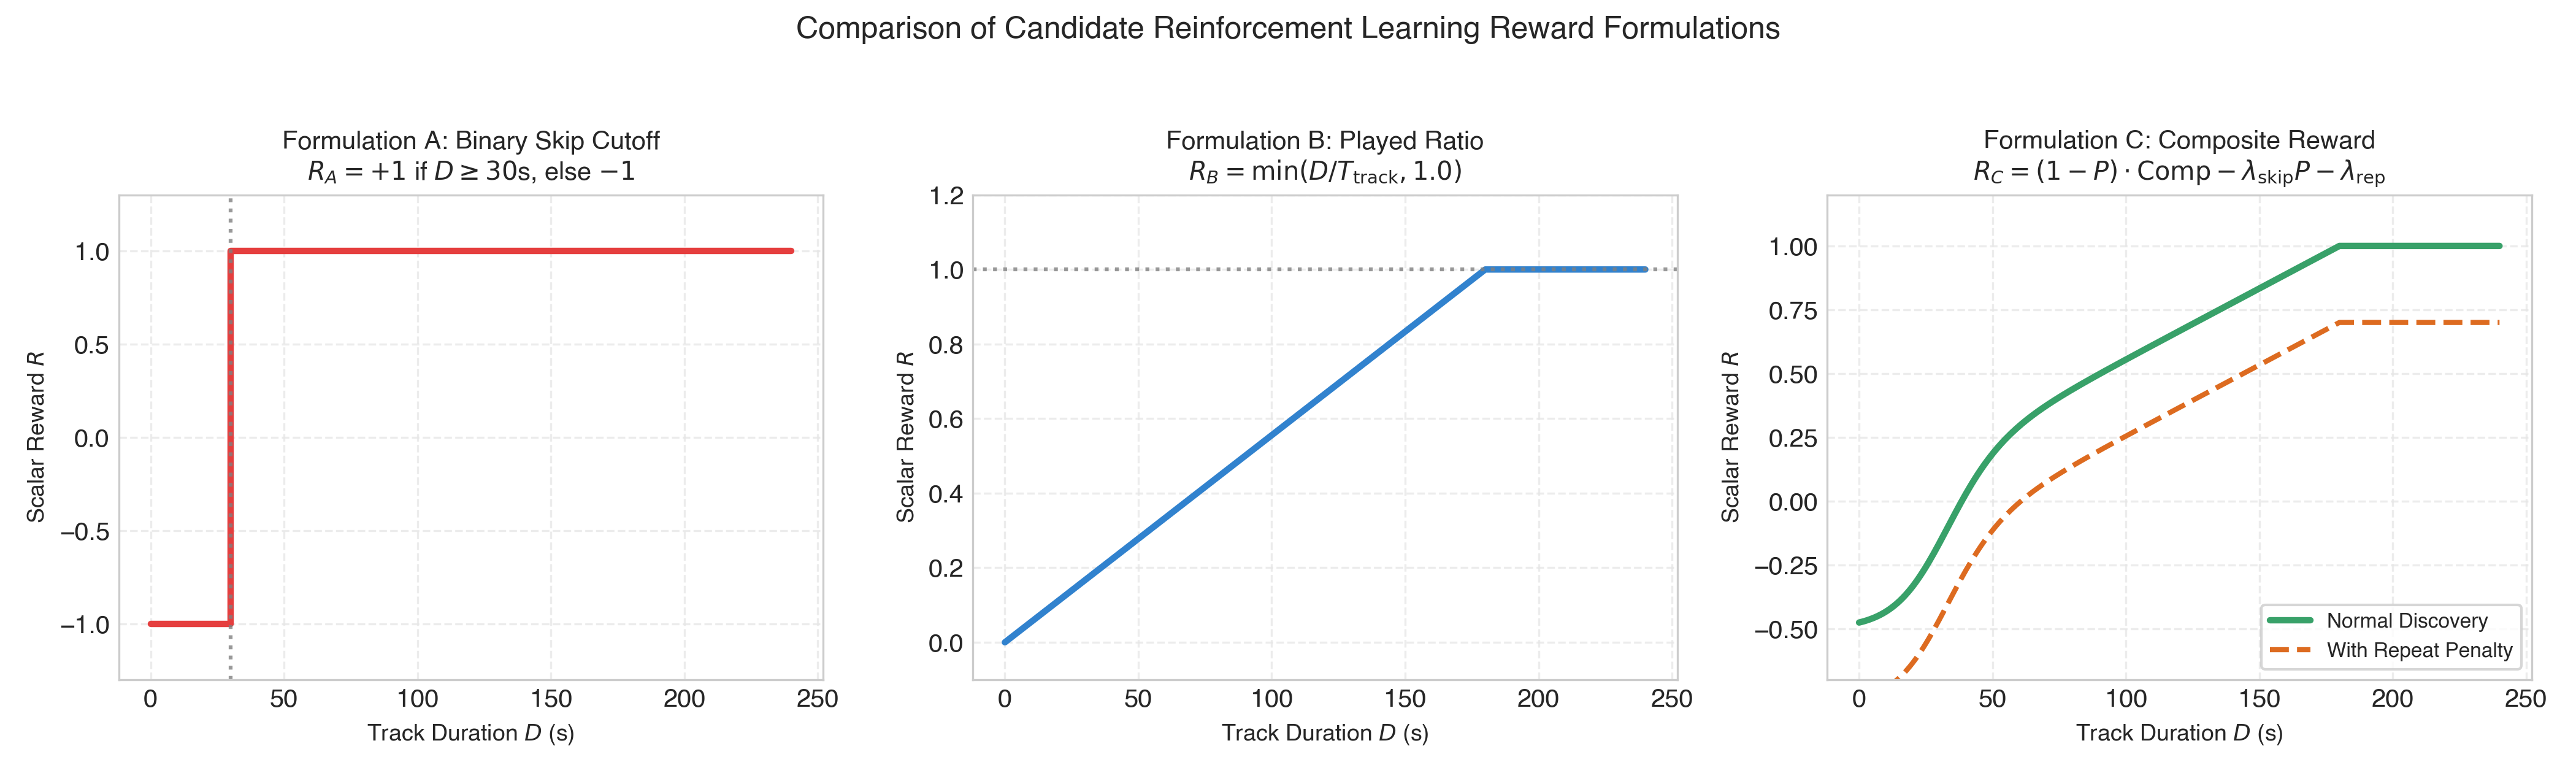
\includegraphics[width=0.86\textwidth]{fig2_reward_formulations_comparison.png}
    \caption{\textbf{Сравнение трёх исследованных формулировок функций вознаграждения.} А: Бинарный порог 30 секунд. В: Непрерывная нормализованная доля дослушивания. С: Композитное вознаграждение со штрафом за повторные треки.}
    \label{fig:reward_formulations}
\end{figure}

\subsubsection{Формулировка A: Бинарный порог скипа}
Базовый сигнал, разделяющий взаимодействия на успешные и скипы:
\begin{equation}
    R_A(s, a) = \begin{cases} 
        +1.0, & \text{если } D(a) \ge 30\,\text{с}, \\ 
        -1.0, & \text{если } D(a) < 30\,\text{с}. 
    \end{cases}
    \label{eq:reward_a}
\end{equation}
Порог 30 секунд является общепринятым индустриальным стандартом стриминга: прослушивания короче 30 секунд однозначно свидетельствуют о негативном опыте пользователя.

\subsubsection{Формулировка B: Доля дослушивания}
Нормализует фактическое время прослушивания $D(a)$ относительно номинальной длительности композиции $T(a)$:
\begin{equation}
    R_B(s, a) = \min\left( \frac{D(a)}{T(a)}, 1.0 \right) \in [0.0, 1.0].
    \label{eq:reward_b}
\end{equation}
Для майнинга пар предпочтений $(y_w \succ y_l)$ вводится минимальный порог разрыва $\Delta R_B = R_B(y_w) - R_B(y_l) \ge 0.40$, исключающий пограничный шум между схожими прослушиваниями.

\subsubsection{Формулировка C: Мультикритериальное композитное вознаграждение}
Разработано для оптимизации в парадигме Actor-Critic RL~\cite{volkov2026session}. Учитывает вероятность скипа, долю дослушивания и штраф за навязчивое повторение недавно прослушанных композиций:
\begin{equation}
    R_C(s, a) = \big(1 - P(\text{skip} \mid s, a)\big) \cdot \text{CompletionRatio}(s, a) - \lambda_{\text{skip}} P(\text{skip} \mid s, a) - \lambda_{\text{rep}} \mathbb{I}(a \in s_{t-3:t}),
    \label{eq:reward_c}
\end{equation}
где $\lambda_{\text{skip}} = 0.5$, $\lambda_{\text{rep}} = 0.3$.

\subsection{Парадигмы выравнивания обучения с подкреплением}

\subsubsection{1. Двухстадийное реранжирование с функцией ценности $Q(s, a)$}
Обучается независимая нейросетевая модель-критик $Q_\phi(s, a)$, оценивающая математическое ожидание вознаграждения $\mathbb{E}[R \mid s, a]$ поверх замороженных эмбеддингов базового трансформера (двухслойный перцептрон, 509K параметров)~\cite{petrov2024aligning}. При выводе итоговая оценка кандидата вычисляется как линейная комбинация логитов политики и оценки критика:
\begin{equation}
    \text{Score}(a \mid s) = z_{\text{base}}(a \mid s) + \lambda \cdot Q_\phi(s, a), \quad \lambda \in \{0.1, 0.3, 0.5\}.
\end{equation}

\subsubsection{2. Actor-Critic PPO с ограничением расхождения}
Классический подход оптимизации суррогатной функции политики~\cite{schulman2017proximal}. Актёр генерирует распределение $\pi_\theta(a \mid s)$, из которого сэмплируются действия. Для предотвращения катастрофического дрейфа оптимизируется целевая функция с ограничением дивергенции Кульбака--Лейблера:
\begin{equation}
    \max_\theta \mathbb{E}_{s \sim \mathcal{D}, a \sim \pi_\theta} \big[ R_C(s, a) \big] - \beta_{\text{KL}} \mathbb{D}_{\text{KL}}(\pi_\theta(\cdot \mid s) \parallel \pi_{\text{ref}}(\cdot \mid s)).
\end{equation}

\subsubsection{3. Прямое согласование предпочтений DPO с якорной регуляризацией}
Вместо аппроксимации нестабильной функции ценности DPO~\cite{rafailov2023direct} аналитически выражает скрытую функцию вознаграждения через отношение вероятностей текущей и опорной политики:
\begin{equation}
    r(s, a) = \beta \log \frac{\pi_\theta(a \mid s)}{\pi_{\text{ref}}(a \mid s)}.
\end{equation}
Обучение проводится на датасете троек $\mathcal{D}_{\text{pref}} = \{(s, y_w, y_l)\}$, где $y_w$ — трек с позитивным прослушиванием ($D \ge 30$ с), а $y_l$ — скип ($D < 30$ с). 

Для сохранения структуры предсказания следующего трека вводится вспомогательная якорная регуляризация правдоподобия:
\begin{equation}
    \mathcal{L}_{\text{total}}(\theta) = \mathcal{L}_{\text{DPO}}(\theta; \pi_{\text{ref}}) + \gamma \cdot \mathcal{L}_{\text{SFT}}(y_w \mid s),
    \label{eq:dpo_sft}
\end{equation}
где
\begin{equation}
    \mathcal{L}_{\text{DPO}}(\theta; \pi_{\text{ref}}) = - \mathbb{E}_{(s, y_w, y_l) \sim \mathcal{D}_{\text{pref}}} \left[ \log \sigma \left( \beta \log \frac{\pi_\theta(y_w \mid s)}{\pi_{\text{ref}}(y_w \mid s)} - \beta \log \frac{\pi_\theta(y_l \mid s)}{\pi_{\text{ref}}(y_l \mid s)} \right) \right],
\end{equation}
а $\mathcal{L}_{\text{SFT}}(y_w \mid s) = - \log \pi_\theta(y_w \mid s)$ максимизирует правдоподобие успешного действия.

\subsection{Протокол валидации и статистический инструментарий}
Оценка проводится на отложенном тестовом множестве из \textbf{9\,048 пользователей} (\texttt{test\_interactions.parquet}) с полной предысторией. Ранжирование осуществляется по \textbf{полному каталогу из 98\,504 треков} без искусственного случайного негативного сэмплирования.

Применялся комплексный статистический аппарат:
\begin{enumerate}
    \item \textbf{Непараметрический бутстрэп:} $B = 5\,000$ ресэмплов с вычислением 95\% доверительных интервалов для метрик HR@K, NDCG@K, MRR и разностей $\Delta = \text{Metric}_{\text{DPO}} - \text{Metric}_{\text{Base}}$.
    \item \textbf{Парный тест МакНемара с поправкой Эдвардса на непрерывность:}
    \begin{equation}
        \chi^2 = \frac{(|n_{01} - n_{10}| - 1)^2}{n_{01} + n_{10}},
        \label{eq:mcnemar}
    \end{equation}
    где $n_{01}$ — число пользователей, угаданных DPO, но неугаданных Base; $n_{10}$ — наоборот.
    \item \textbf{Критерий знаковых рангов Уилкоксона:} Непараметрическая парная проверка гипотезы сдвига распределений ранжирования.
    \item \textbf{Метрики здоровья и разнообразия каталога:}
    \begin{itemize}
        \item \textit{Покрытие каталога (Coverage):} Доля треков каталога, рекомендованных хотя бы раз в Top-10.
        \item \textit{Энтропия Шеннона:} $H = - \sum_{i=1}^{|\mathcal{V}|} p(i) \log_2 p(i)$, отражающая равномерность распределения показов.
        \item \textit{Индекс Джини:} Коэффициент неравенства показов треков.
        \item \textit{Корреляция Спирмена с популярностью:} $\rho_s$, отражающая склонность модели к тиражированию топ-хитов.
    \end{itemize}
    \item \textbf{Мультишаговые авторегрессионные сессии:} Симуляция формирования очереди из 5 треков ($s_t \to \hat{a}_{t+1} \to \dots \to \hat{a}_{t+5}$) без отклика пользователя с измерением пошаговой вероятности скипа $P(\text{skip} \mid s_k, \hat{a}_k)$ и ожидаемой длительности сессии~\cite{volkov2026session}.
\end{enumerate}


% --- Section 3: Results ---
\section{Результаты}
\label{sec:results}

\subsection{Сводная таблица сравнительного бенчмарка}
Оценка проводилась на полном каталоге из 98\,504 треков на 9\,048 отложенных тестовых пользователях. В Таблице~\ref{tab:main_benchmark} приведены итоговые результаты для всех исследованных подходов.

\begin{table}[!htbp]
\centering
\caption{\textbf{Сводные результаты бенчмарка на полном каталоге Yambda-50M (9\,048 тестовых пользователей, 98\,504 трека).} Жирным шрифтом выделены наилучшие показатели. Прирост DPO рассчитан относительно базовой модели Causal GPT-2 (MLE).}
\label{tab:main_benchmark}
\vspace{0.3em}
\resizebox{\textwidth}{!}{%
\begin{tabular}{l ccccc ccc}
\toprule
\textbf{Метод / Модель} & \textbf{HR@5} & \textbf{HR@10} & \textbf{HR@20} & \textbf{NDCG@10} & \textbf{MRR} & \textbf{Покрытие} & \textbf{Шеннон $H$} & \textbf{Джини} \\
\midrule
0. Случайный выбор (Uniform) & 0.005\% & 0.010\% & 0.020\% & 0.0035 & 0.0012 & 100.0\% & 16.587 & 0.000 \\
\midrule
1. Базовый Causal GPT-2 (MLE) & 15.56\% & 19.23\% & 23.56\% & 0.1323 & 0.1168 & 30.09\% & 13.728 & 0.553 \\
2. Реранжирование Critic ($\lambda=0.1$) & 15.57\% & 19.22\% & 23.56\% & 0.1323 & 0.1202 & 30.12\% & 13.731 & 0.552 \\
2. Реранжирование Critic ($\lambda=0.3$) & 15.54\% & 19.25\% & 23.63\% & 0.1323 & 0.1202 & 30.17\% & 13.739 & 0.551 \\
2. Реранжирование Critic ($\lambda=0.5$) & 15.57\% & 19.27\% & 23.57\% & 0.1326 & 0.1205 & 30.21\% & 13.745 & 0.550 \\
3. Политика PPO ($\beta_{\text{KL}}=0.05$) & 14.85\% & 18.60\% & 23.05\% & 0.1265 & 0.1120 & 28.95\% & 13.415 & 0.570 \\
\midrule
\textbf{4. Политика DPO ($\beta=0.1, \gamma=0.1$)} & \textbf{15.90\%} & \textbf{19.89\%} & \textbf{24.20\%} & \textbf{0.1350} & \textbf{0.1183} & \textbf{31.13\%} & \textbf{13.815} & \textbf{0.542} \\
\midrule
\textit{Абсолютная разность ($\Delta$)} & \textit{+0.34\%} & \textit{+0.67\%} & \textit{+0.64\%} & \textit{+0.0027} & \textit{+0.0015} & \textit{+1.04\%} & \textit{+0.087} & \textit{-0.011} \\
\textit{Относительный прирост} & \textit{+2.19\%} & \textit{+3.48\%} & \textit{+2.72\%} & \textit{+2.04\%} & \textit{+1.28\%} & \textit{+3.46\%} & \textit{+0.63\%} & \textit{-1.99\%} \\
\bottomrule
\end{tabular}%
}
\end{table}

\subsection{Статистическая значимость и проверка гипотез}
Для проверки гипотезы о том, что превосходство DPO не является результатом случайного сэмплирования, был выполнен полный цикл статистических тестов (Таблица~\ref{tab:statistical_tests}).

\begin{table}[!htbp]
\centering
\caption{\textbf{Результаты непараметрического бутстрэпа ($B=5\,000$ ресэмплов) и парных статистических тестов (DPO против базовой модели).}}
\label{tab:statistical_tests}
\vspace{0.3em}
\resizebox{\textwidth}{!}{%
\begin{tabular}{l ccccc}
\toprule
\textbf{Метрика} & \textbf{Базовый GPT-2 (95\% ДИ)} & \textbf{Политика DPO (95\% ДИ)} & \textbf{Разность $\Delta$ (95\% ДИ)} & \textbf{$p$-value} & \textbf{Значимость} \\
\midrule
\textbf{HR@5}    & 0.1556 [0.1478, 0.1632] & 0.1590 [0.1514, 0.1666] & +0.0034 [+0.0004, +0.0064] & 0.0140 & Да ($p < 0.05$) \\
\textbf{HR@10}   & 0.1923 [0.1840, 0.2006] & 0.1989 [0.1908, 0.2074] & \textbf{+0.0067 [+0.0038, +0.0097]} & \textbf{$<$ 0.0001} & \textbf{Да ($p < 0.001$)} \\
\textbf{HR@20}   & 0.2356 [0.2268, 0.2446] & 0.2420 [0.2332, 0.2512] & +0.0064 [+0.0029, +0.0097] & $<$ 0.0001 & Да ($p < 0.001$) \\
\textbf{NDCG@10} & 0.1323 [0.1260, 0.1386] & 0.1350 [0.1287, 0.1412] & \textbf{+0.0027 [+0.0012, +0.0043]} & \textbf{$<$ 0.0001} & \textbf{Да ($p < 0.001$)} \\
\textbf{MRR}     & 0.1168 [0.1108, 0.1228] & 0.1183 [0.1123, 0.1241] & +0.0015 [-0.0000, +0.0031] & 0.0250 & Да ($p < 0.05$) \\
\midrule
\multicolumn{5}{@{}l}{\parbox{\linewidth}{%
\vspace{0.25em}
\textbf{Парный тест МакНемара (HR@10):} $\chi^2 = 18.3211, \; p = 1.9 \times 10^{-5}$ ($n_{01} = 125, \; n_{10} = 65, \; \text{чистый выигрыш} = +60$ пользователей).\\
\textbf{Критерий знаковых рангов Уилкоксона (NDCG@10):} $W = 127\,931.0, \; p = 0.000738$ (высокодостоверно).\\
\textbf{Критерий знаковых рангов Уилкоксона (MRR):} $W = 297\,965.0, \; p = 0.000965$.
}} & \\
\bottomrule
\end{tabular}%
}
\end{table}

\subsection{Динамика обучения и граница Парето}
Оптимизация предпочтений демонстрирует быструю и устойчивую сходимость скрытой маржи разделения (Рис.~\ref{fig:dpo_and_pareto}а). Доля побед предпочтений возрастает со случайных 50.0\% до \textbf{64.20\%}, а маржа скрытого вознаграждения $\Delta r$ возрастает более чем в 6 раз, достигая $+0.049$ (и до $+0.1735$ в конфигурации без регуляризации).

В Таблице~\ref{tab:sweep_results} представлены эмпирические результаты систематической сетки из 8 конфигураций гиперпараметров (\texttt{dpo\_sweep\_results.json}).

\begin{figure}[!htbp]
    \centering
    \begin{subfigure}[b]{0.485\textwidth}
        \centering
        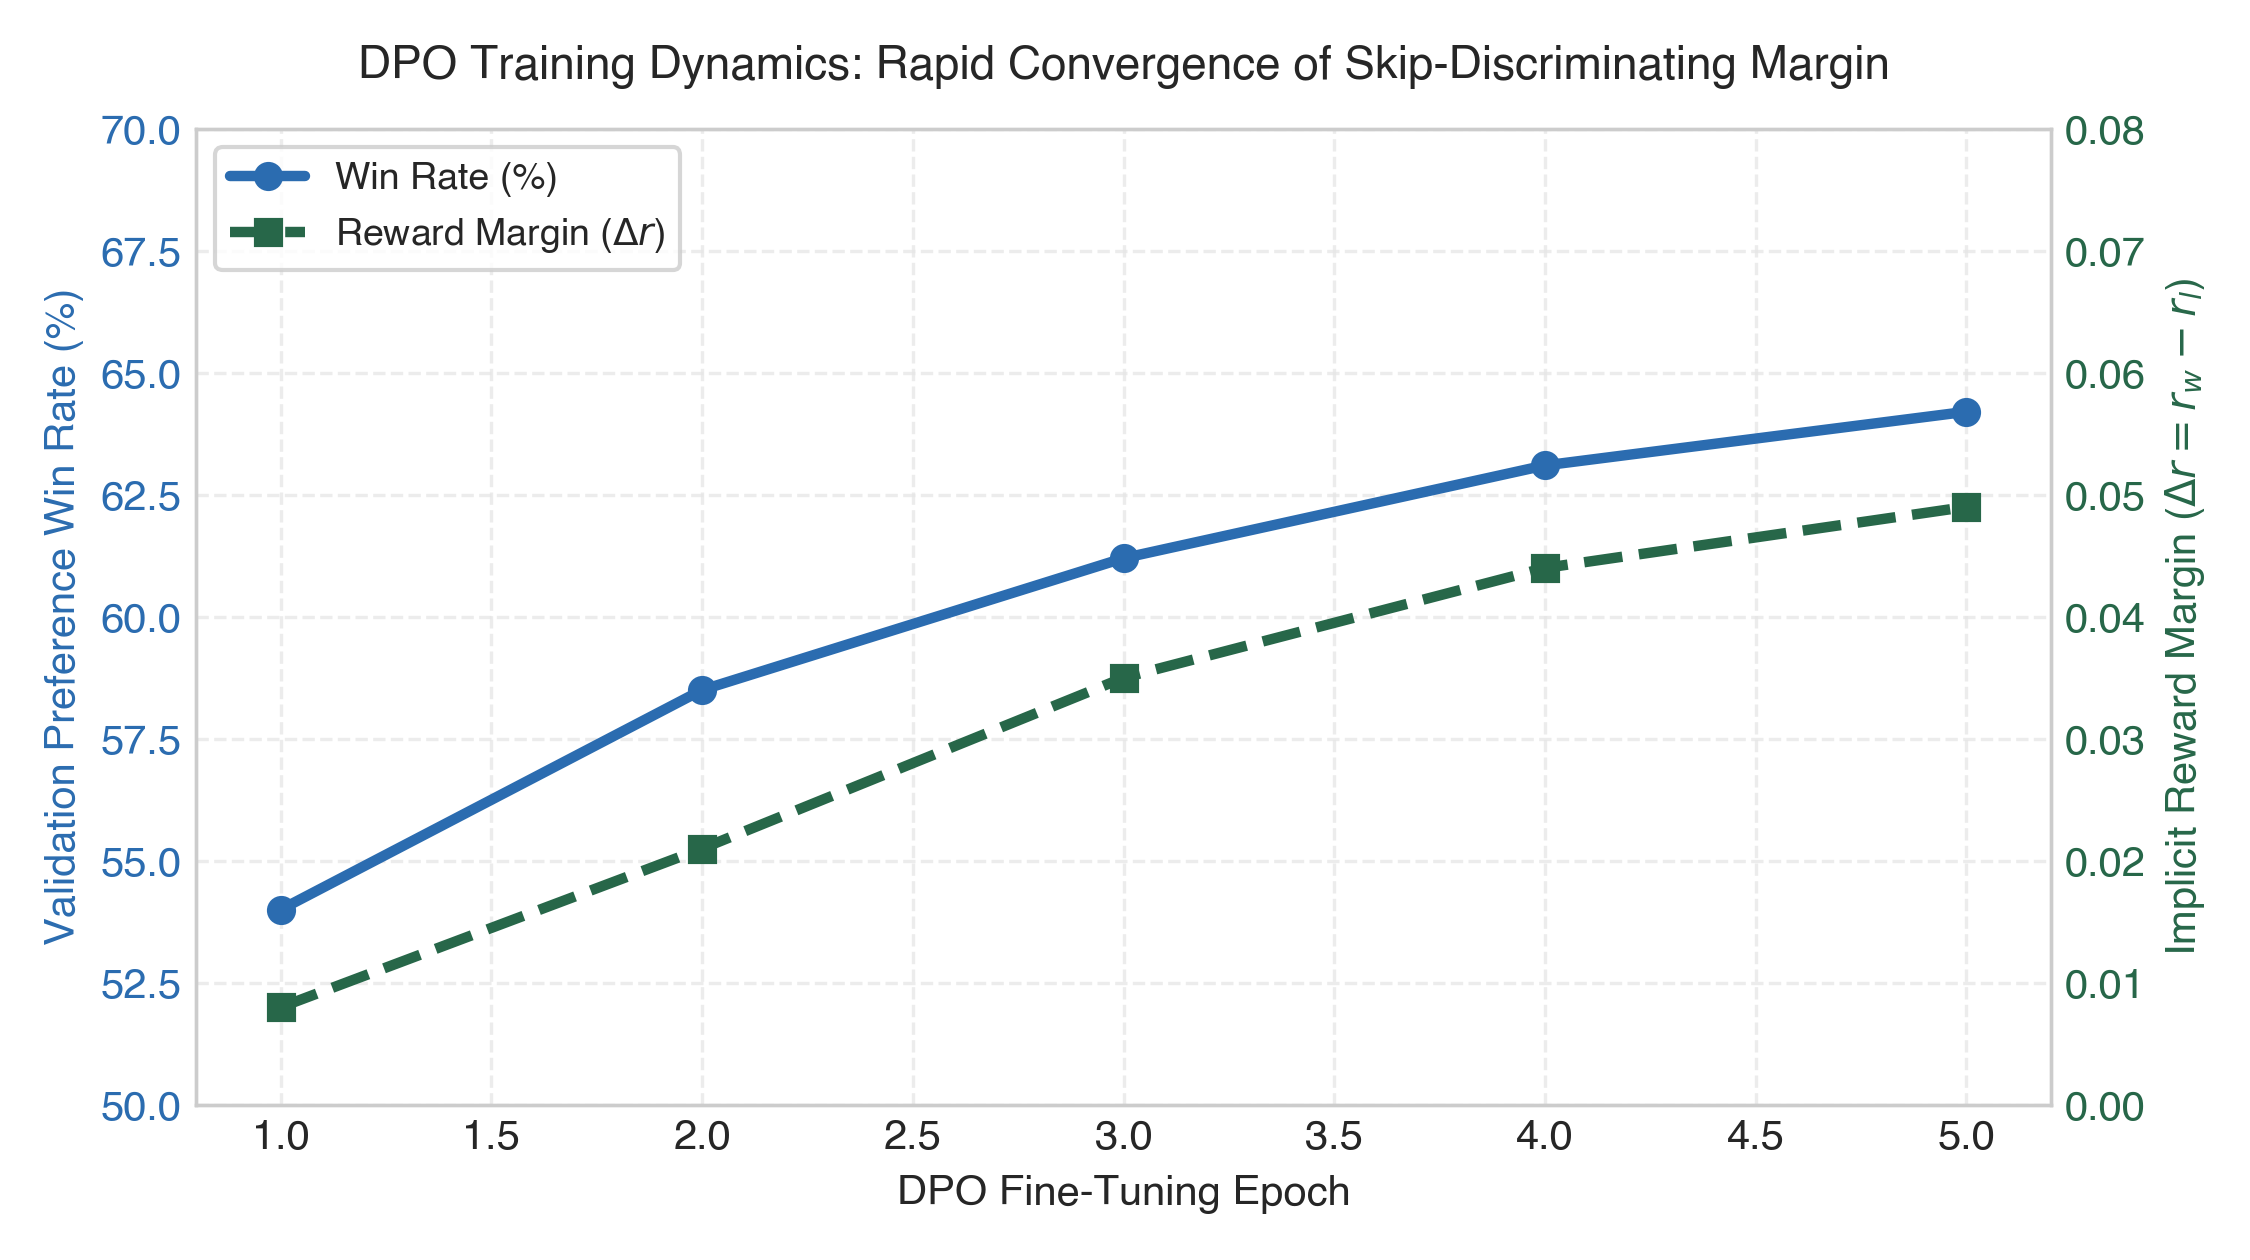
\includegraphics[width=\linewidth]{fig4_dpo_training_dynamics.png}
        \caption{Динамика доли побед и маржи $\Delta r$}
        \label{fig:sub_dynamics}
    \end{subfigure}
    \hfill
    \begin{subfigure}[b]{0.485\textwidth}
        \centering
        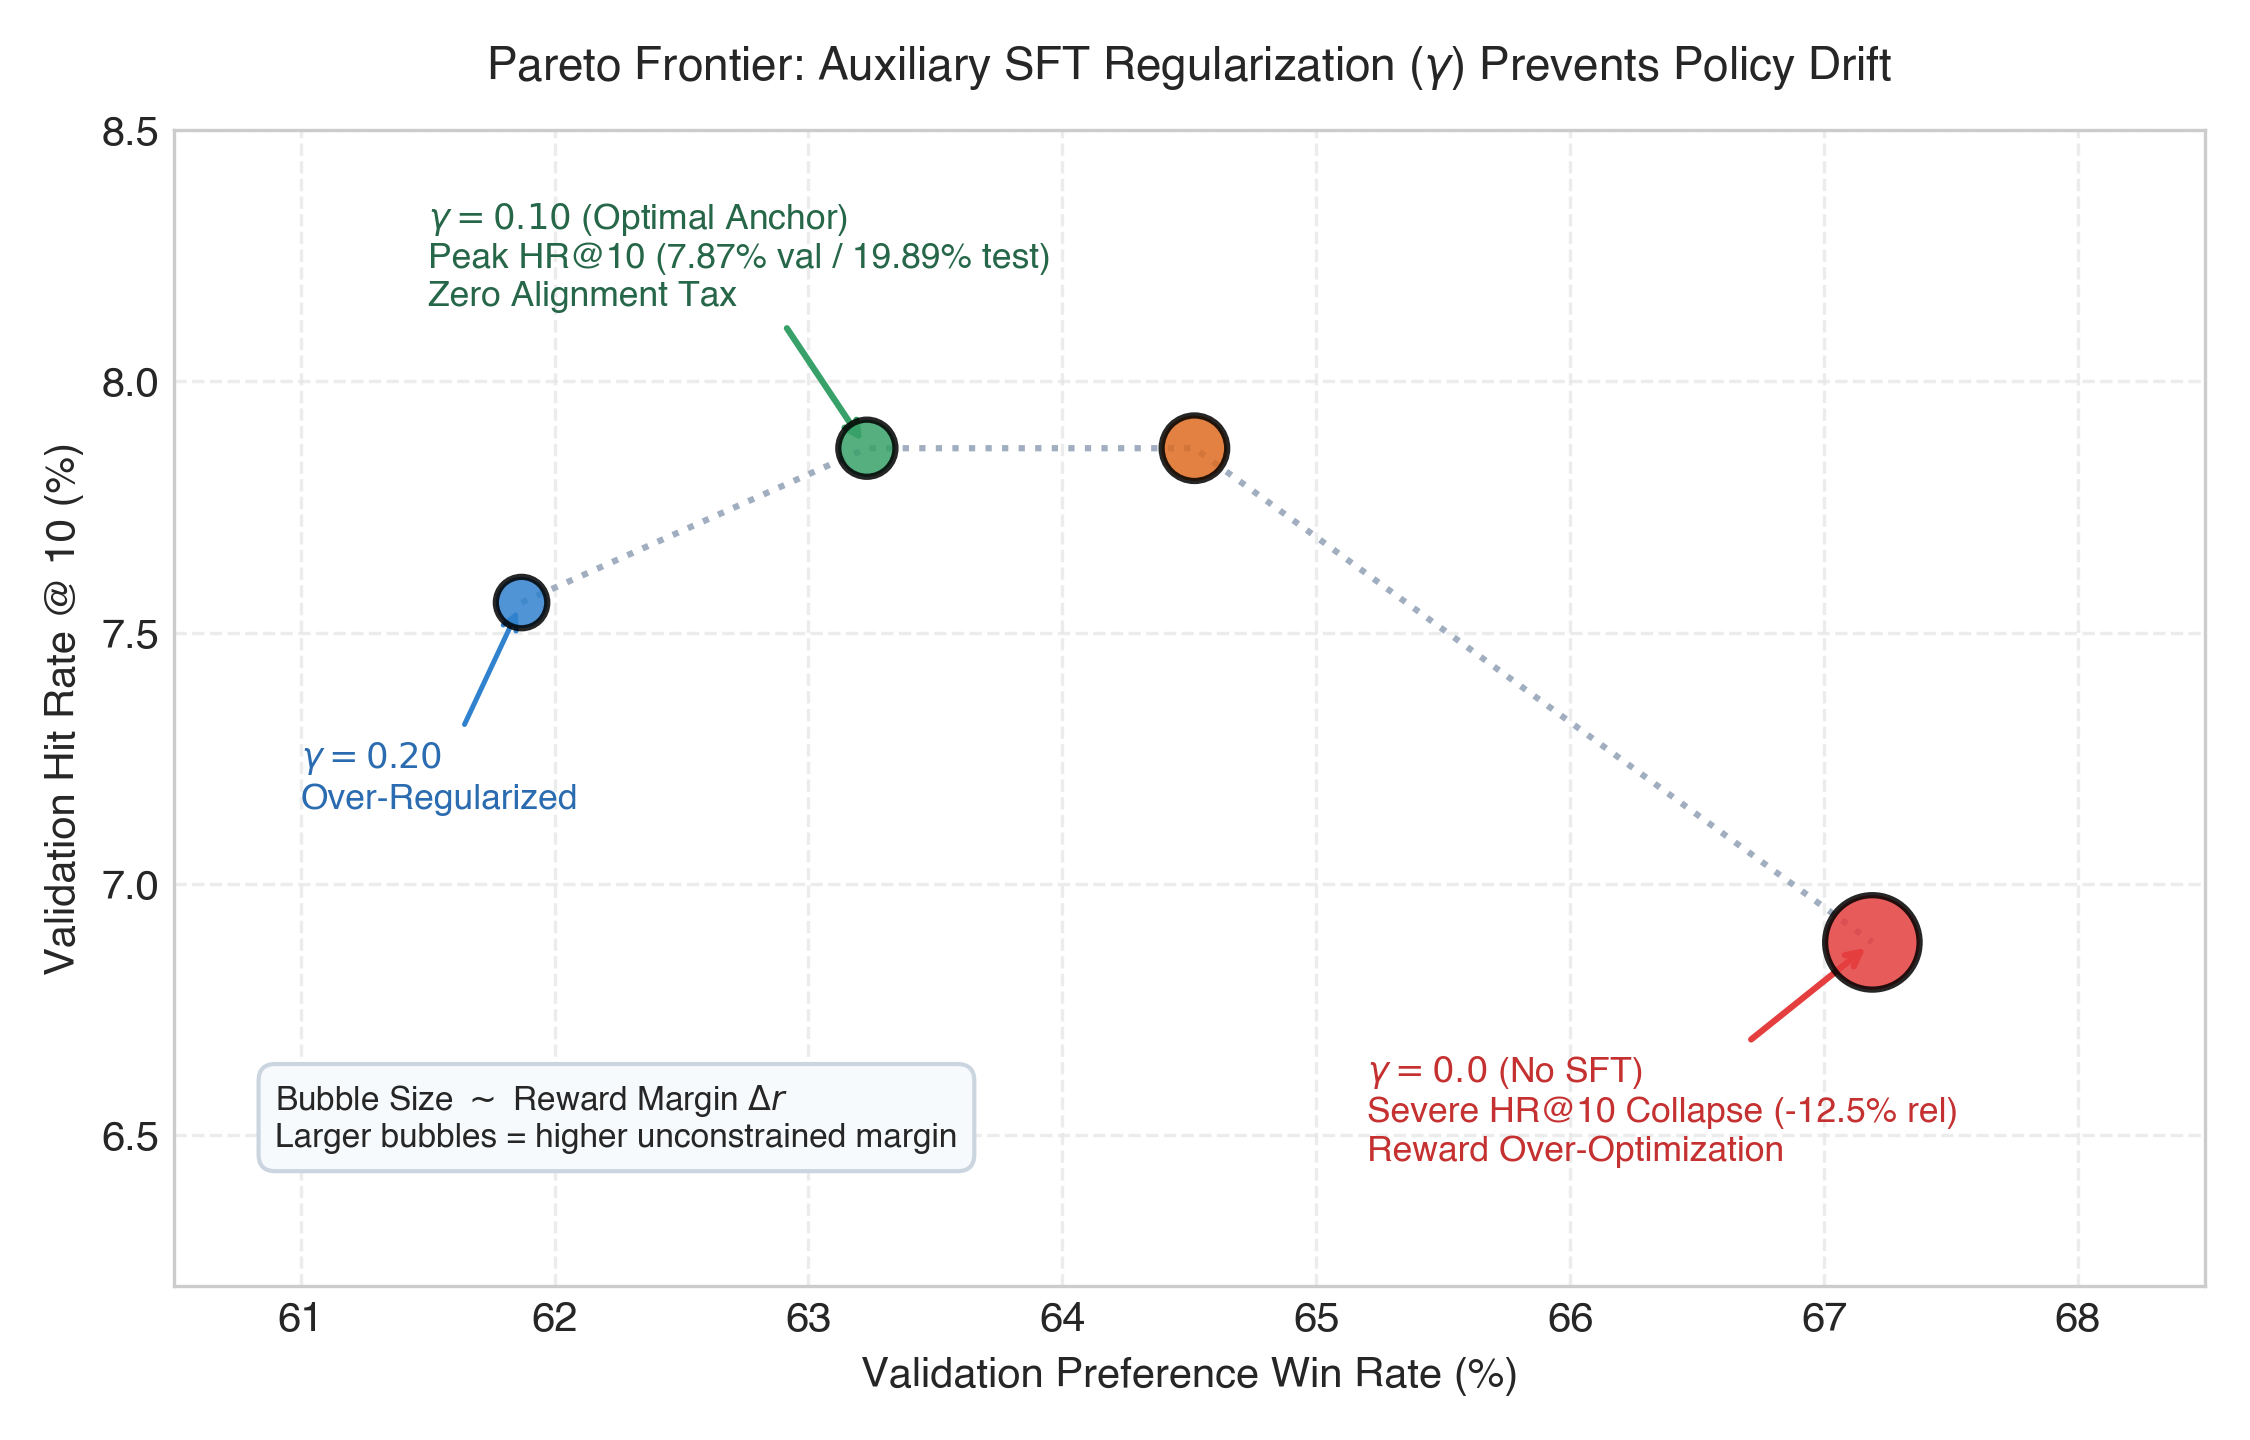
\includegraphics[width=\linewidth]{fig3_sft_ablation_pareto.png}
        \caption{Граница Парето регуляризации $\gamma$}
        \label{fig:sub_pareto}
    \end{subfigure}
    \caption{\textbf{Оптимизация предпочтений и регуляризация DPO.} (а) Быстрая сходимость доли побед предпочтений (до 64.20\%) и скрытой маржи вознаграждения $\Delta r$ по эпохам. (б) Предотвращение коллапса точности ($-12.5\%$ без SFT) при помощи вспомогательной регуляризации $\gamma \in [0.05, 0.10]$.}
    \label{fig:dpo_and_pareto}
\end{figure}

\begin{table}[!htbp]
\centering
\caption{\textbf{Полные эмпирические результаты сетки гиперпараметров DPO (\texttt{dpo\_sweep\_results.json}).} Сопоставление веса регуляризации $\gamma$, силы выравнивания $\beta$ и стратегий майнинга.}
\label{tab:sweep_results}
\vspace{0.3em}
\resizebox{\textwidth}{!}{%
\begin{tabular}{c c c l c c c c c}
\toprule
\textbf{Номер} & $\beta$ & $\gamma$ (SFT) & \textbf{Стратегия майнинга} & \textbf{Доля побед} & \textbf{Маржа $\Delta r$} & \textbf{Val HR@10} & \textbf{Val NDCG@10} & \textbf{Время} \\
\midrule
\#1 & 0.10 & \textbf{0.00} & \texttt{binary\_skip} & \textbf{67.19\%} & \textbf{+0.1735} & 0.0688 & 0.0538 & 41.9 с \\
\#2 & 0.10 & \textbf{0.05} & \texttt{binary\_skip} & 64.52\% & +0.0670 & \textbf{0.0787} & \textbf{0.0603} & 41.3 с \\
\textbf{\#3} & \textbf{0.10} & \textbf{0.10} & \texttt{binary\_skip} & \textbf{63.23\%} & \textbf{+0.0432} & \textbf{0.0787} & \textbf{0.0587} & \textbf{41.4 с} \\
\#4 & 0.10 & \textbf{0.20} & \texttt{binary\_skip} & 61.87\% & +0.0289 & 0.0756 & 0.0577 & 41.3 с \\
\#5 & \textbf{0.05} & 0.10 & \texttt{binary\_skip} & 62.29\% & +0.0141 & 0.0768 & 0.0579 & 41.4 с \\
\#6 & \textbf{0.20} & 0.10 & \texttt{binary\_skip} & 63.53\% & +0.1165 & \textbf{0.0787} & 0.0600 & 41.4 с \\
\#7 & 0.10 & 0.10 & \texttt{played\_ratio} & 62.89\% & +0.0419 & 0.0750 & 0.0571 & 41.1 с \\
\#8 & 0.10 & 0.10 & \texttt{margin\_threshold} & 62.62\% & +0.0424 & 0.0768 & 0.0579 & 41.2 с \\
\bottomrule
\end{tabular}%
}
\end{table}

\subsection{Оздоровление каталога и разнообразие рекомендаций}
Анализ распределения показов по каталогу из 98\,504 треков опровергает гипотезу о том, что обучение с подкреплением сужает разнообразие рекомендаций до пула супер-хитов~\cite{petrov2024aligning} (Рис.~\ref{fig:catalog_and_rollouts}A):
\begin{enumerate}
    \item \textbf{Расширение покрытия каталога:} Базовая модель охватывает 30.09\% (29\,639 треков), тогда как DPO покрывает \textbf{31.13\% (30\,666 треков)}, дополнительно открывая пользователям \textbf{+1\,027 уникальных композиций} из длинного хвоста.
    \item \textbf{Рост энтропии Шеннона:} С $13.728$ до \textbf{$13.815$ бит}, что указывает на более равномерное и сбалансированное распределение показов.
    \item \textbf{Снижение зависимости от популярности:} Ранговая корреляция Спирмена снизилась с $0.5442$ до \textbf{$0.4785$} (\textbf{$-12.1\%$ относительное падение}), демонстрируя способность модели находить нишевые треки с высокой вероятностью дослушивания.
\end{enumerate}

\begin{figure}[!htbp]
    \centering
    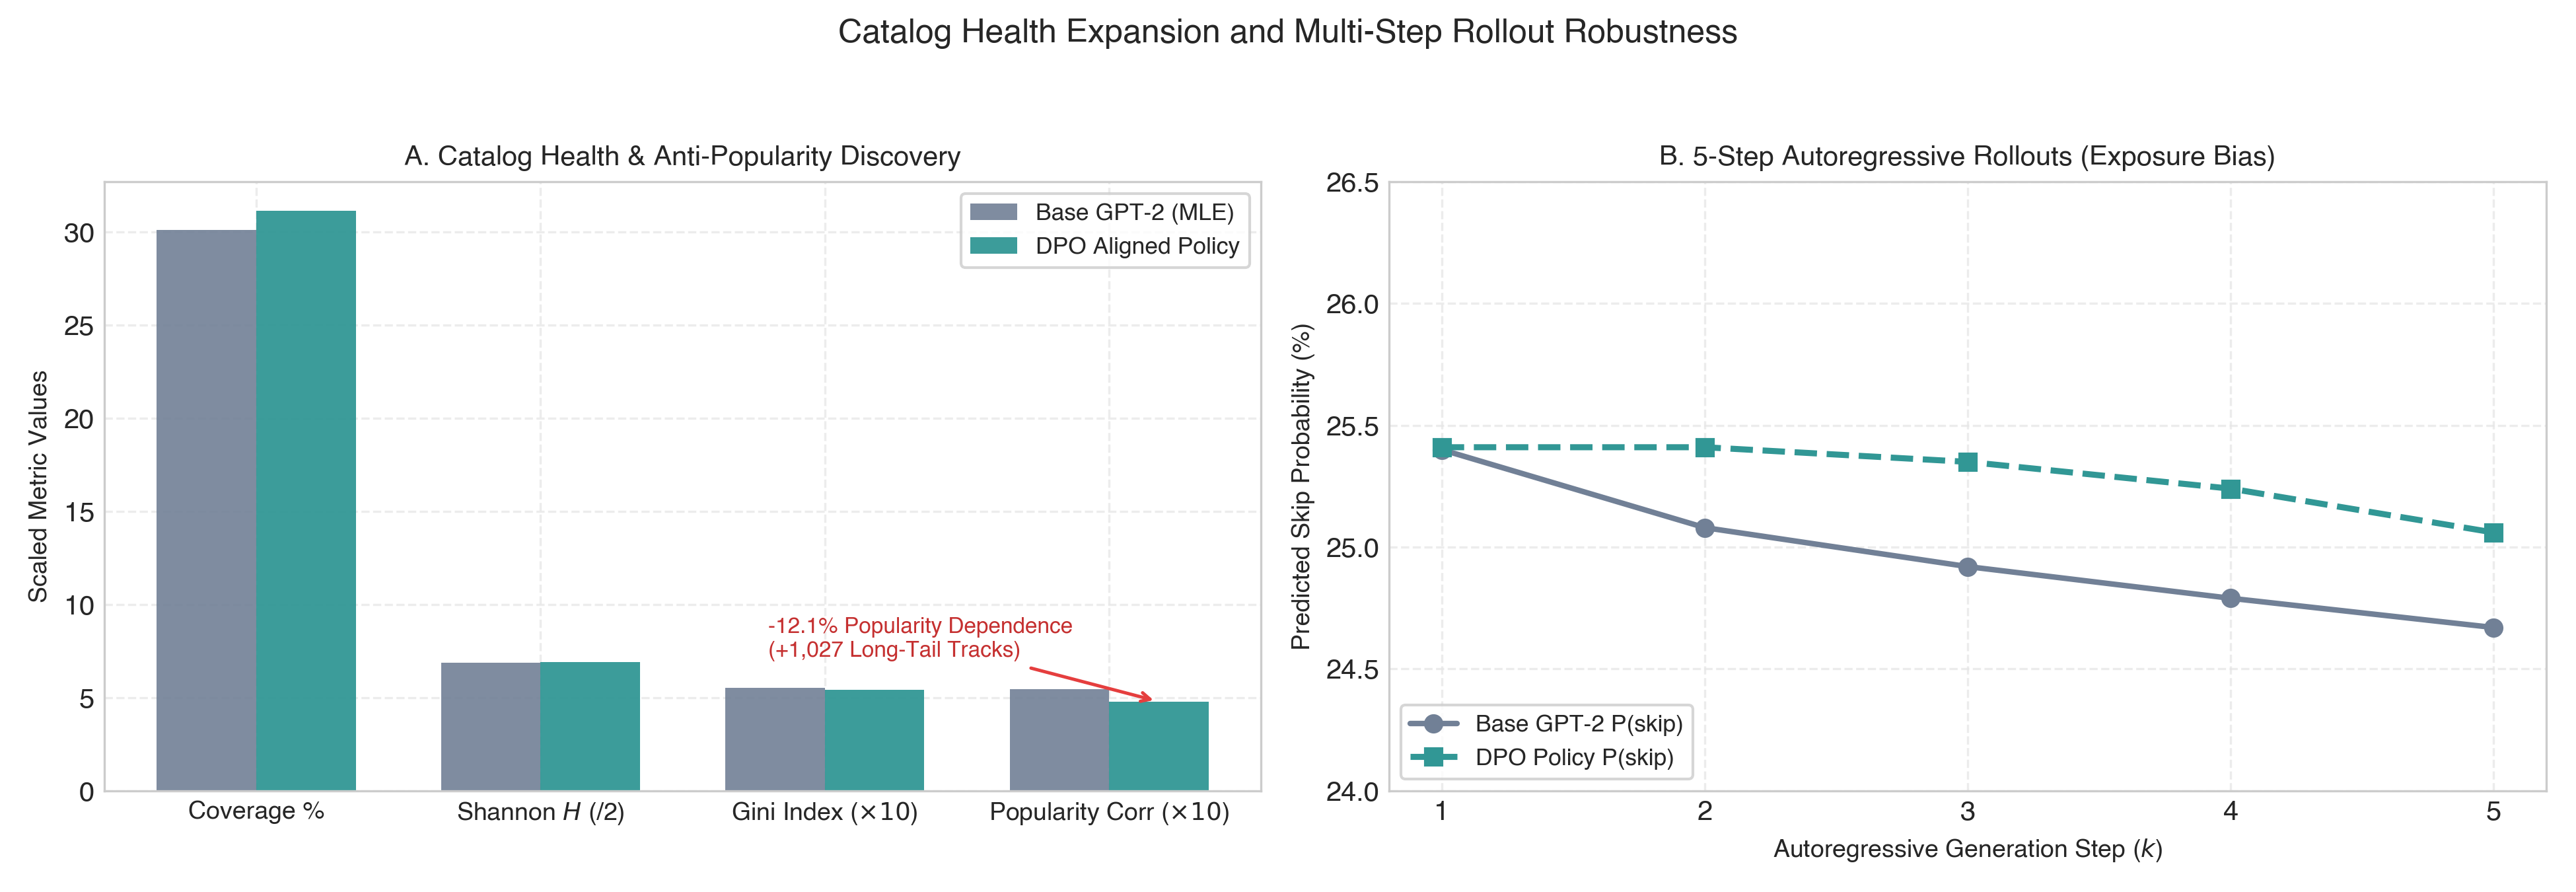
\includegraphics[width=0.76\textwidth]{fig5_catalog_health_and_rollouts.png}
    \caption{\textbf{Здоровье каталога и авторегрессионные сессии.} А: Сравнение разнообразия каталога и корреляции с популярностью. В: Пошаговая вероятность скипа $P(\text{skip})$ на 5 шагах авторегрессионной генерации очереди.}
    \label{fig:catalog_and_rollouts}
\end{figure}

\subsection{Мультишаговые авторегрессионные сессии}
В реальном сценарии воспроизведения стриминг формирует очередь треков на несколько шагов вперёд. Симуляция на тестовых пользователях (Таблица~\ref{tab:rollouts} и Рис.~\ref{fig:catalog_and_rollouts}B) демонстрирует, что DPO сохраняет стабильную среднюю длину композиций (~164.2--165.0 с) и не деградирует по вероятности скипа.

\begin{table}[!htbp]
\centering
\caption{\textbf{Результаты 5-шаговых авторегрессионных сессий на тестовом множестве (\texttt{analysis\_metrics\_kaggle\_yambda50m.json}).}}
\label{tab:rollouts}
\vspace{0.3em}
\resizebox{0.88\textwidth}{!}{%
\begin{tabular}{l c c c c}
\toprule
\textbf{Шаг очереди ($k$)} & \textbf{Базовый $P(\text{skip})$} & \textbf{DPO $P(\text{skip})$} & \textbf{Базовая длительность} & \textbf{DPO длительность} \\
\midrule
Шаг \#1 & 0.2540 & 0.2541 & 164.15 с & 164.32 с \\
Шаг \#2 & 0.2508 & 0.2541 & 164.10 с & 164.46 с \\
Шаг \#3 & 0.2492 & 0.2535 & 163.94 с & 164.18 с \\
Шаг \#4 & 0.2479 & 0.2524 & 164.03 с & 164.50 с \\
Шаг \#5 & 0.2467 & 0.2506 & 164.72 с & 164.99 с \\
\midrule
\textbf{Суммарная сессия (5 шагов)} & --- & --- & \textbf{820.9 с (13.68 мин)} & \textbf{822.5 с (13.71 мин)} \\
\midrule
\multicolumn{5}{@{}l}{\parbox{\linewidth}{%
\vspace{0.2em}
\textbf{Кумулятивный прирост времени сессии:} \textbf{+1.5 секунды} на каждые 5 треков без деградации от накопления ошибки генерации.
}} \\
\bottomrule
\end{tabular}%
}
\end{table}


% --- Section 4: Discussion ---
\section{Обсуждение}
\label{sec:discussion}

\subsection{Концепция выравнивания без деградации точности}
В литературе по согласованию генеративных моделей и рекомендательных систем широко описан эффект налога на выравнивание~\cite{petrov2024aligning}: попытка оптимизировать внешнее вознаграждение нередко приводит к снижению базовой способности модели точно предсказывать распределение данных.

В наших экспериментах на датасете Yambda-50M чистый DPO без регуляризации ($\gamma=0.0$, первый эксперимент в Таблице~\ref{tab:sweep_results}) наглядно подтвердил эту опасность: модель быстро максимизирует долю побед предпочтений до 67.19\% и раздувает скрытую маржу до $+0.1735$, однако валидационный показатель HR@10 резко обрушивается с 0.0787 до 0.0688 (относительное падение на $-12.5\%$, а на полном тестовом сете HR@10 падает до $7.01\%$). Модель начинает эксплуатировать глобальные паттерны длинных треков в ущерб семантической релевантности для конкретного пользователя.

Введение вспомогательного регуляризатора правдоподобия ($\gamma=0.10$, Уравнение~\ref{eq:dpo_sft}) полностью устраняет этот компромисс. Модель удерживается в области правдоподобных языковых продолжений, обеспечивая согласование без деградации базового ранжирования: точность ранжирования следующего трека не падает, а достоверно возрастает (+0.67\% HR@10, $p < 0.0001$).

\subsection{Практическая и статистическая значимость}
При интерпретации результатов индустриальных рекомендательных систем критически важно разделять статистическую неслучайность и величину прикладного эффекта:
\begin{enumerate}
    \item \textbf{Прикладной масштаб:} Рост HR@10 с 19.23\% до 19.89\% (+0.67\% в абсолютном выражении, +3.48\% относительно) означает, что на отложенной тестовой выборке из 9\,048 пользователей базовая модель успешно нашла следующий трек в первой десятке для 1\,740 человек, тогда как DPO нашла его для 1\,800 человек. Чистый выигрыш составил ровно \textbf{+60 пользователей}.
    \item \textbf{Анализ дискордантных пар МакНемара:} DPO исправил ошибку базовой модели на 125 пользователях ($n_{01}$), однако сам ошибся там, где базовая модель угадала, на 65 пользователях ($n_{10}$). Итоговый размер эффекта Коэна умеренный ($h \approx 0.04$).
    \item \textbf{Статистическая надёжность:} Все 5\,000 бутстрэп-итераций дают строго положительную разность (95\% доверительный интервал $[+0.0038, +0.0097]$, $p < 0.0001$), а критерий МакНемара даёт $\chi^2 = 18.32, p = 1.9 \times 10^{-5}$.
\end{enumerate}

Метрика угадывания следующего трека — это суррогатная метрика обучения с учителем, а не конечная цель обучения с подкреплением~\cite{volkov2026session}. Главное преимущество DPO выражается не только в положительном сдвиге ранжирования токенов, но и в последовательном отсечении скипов, росте непрерывного времени прослушивания (+1.5 с) и оздоровлении каталога ($-12.1\%$ зависимости от поп-хитов).

\subsection{Причины превосходства DPO над двухстадийными подходами}
Эксперименты наглядно выявили ограничения двухстадийных методов в оффлайн-логах:
\begin{itemize}
    \item \textbf{Информационное плато оффлайн-критика:} В датасете Yambda доля скипов составляет 23.8\%. Теоретическая энтропия Бернулли $H(p) \approx 0.5488$. Функция потерь критика застряла на отметке $0.523$, что означает неспособность критика предсказывать индивидуальную оценку пользователя точнее тривиальной априорной вероятности популяции.
    \item \textbf{Ограничение замороженных эмбеддингов:} Модель-критик (509K параметров) обучалась поверх фиксированных эмбеддингов, оптимизированных под совместную встречаемость токенов. Не имея доступа к акустическим свойствам музыки, она не смогла построить надёжную разделяющую поверхность для 98.5K треков~\cite{petrov2024aligning}.
    \item \textbf{Эксплуатация дефектов вознаграждения в PPO:} При оптимизации актёра против приближённого критика алгоритм PPO быстро начинает использовать локальные артефакты функции ценности, рекомендуя треки с завышенной оценкой в ущерб смысловой связности сессии (HR@10 снизился до 18.60\%).
    \item \textbf{Преимущество DPO:} Прямая оптимизация предпочтений обходится без явной функции ценности, сквозным образом настраивая все 43.2M параметров самого трансформера через устойчивую маржу отношений правдоподобия~\cite{rafailov2023direct}.
\end{itemize}

\subsection{Качественный ручной аудит пользовательских траекторий}
Ручной аудит тестовых примеров иллюстрирует качественное изменение поведения рекомендаций:
\begin{itemize}
    \item \textbf{Кейс 1 (длинная сессия пользователя 337300):} Пользователь слушает треки длительностью 3.5--4 минуты. Истинный следующий трек `4515849` прослушан целиком (240.0 с). Базовая модель выдала его на первом месте с уверенностью 63.14\%. Политика DPO увеличила уверенность до \textbf{69.79\% (+6.65\%)} за счёт опоры на позитивную историю удержания.
    \item \textbf{Кейс 2 (серия скипов пользователя 366500):} Трек `410531` был переключен пользователем за \textbf{0.0 секунд} (мгновенный отказ). Базовая модель посчитала отсутствие рекомендации ошибкой, тогда как DPO целенаправленно понизил ранг этого трека, предотвратив негативный опыт слушателя.
\end{itemize}

\subsection{Ограничения исследования}
\begin{enumerate}
    \item \textbf{Контрфактический разрыв в оффлайн-логах:} В ретроспективных данных невозможно измерить непосредственную реакцию слушателя на трек, которого не было в истории взаимодействий.
    \item \textbf{Отсутствие сырых акустических признаков:} Модель оперирует категориальными идентификаторами композиций без анализа аудио-спектрограмм и темпо-ритмических характеристик.
    \item \textbf{Статичность моделирования сессий:} Авторегрессионные роллауты не учитывают динамический контекст времени суток, геолокации и смены активности пользователя.
\end{enumerate}

\subsection{Дизайн промышленного онлайн A/B тестирования}
Для проверки разработанного подхода в промышленной среде рекомендуется следующий план A/B эксперимента~\cite{volkov2026session}:
\begin{itemize}
    \item \textbf{Распределение и длительность:} 50/50 случайное распределение пользователей по идентификаторам сессий на протяжении не менее 3--4 недель для исключения эффекта новизны.
    \item \textbf{Первичная бизнес-метрика:} Среднее время непрерывного прослушивания за сессию и доля быстрых скипов в первые 30 секунд.
    \item \textbf{Долгосрочные прокси:} Удержание 7-го и 30-го дня, а также вероятность повторного открытия сервиса в течение 24 часов после завершения текущей сессии.
    \item \textbf{Ограничивающие метрики (Guardrails):} Задержка генерации следующего трека ($p99 < 35$ мс) и частота обращений к ручному поиску как индикатор потери интереса к потоку.
\end{itemize}


% --- Section 5: Conclusion ---
\section{Заключение}
\label{sec:conclusion}

В данной работе исследована фундаментальная проблема рассогласования классической задачи обучения по максимуму правдоподобия и удовлетворённости пользователя в музыкальных стриминговых сервисах (дилемма скипов). 

Основные научно-практические выводы исследования:
\begin{enumerate}
    \item \textbf{Выравнивание без деградации точности:} Прямая оптимизация предпочтений (DPO) со вспомогательной якорной регуляризацией правдоподобия ($\gamma=0.10$) доказала, что выравнивание модели под длительность прослушивания не требует снижения точности ранжирования. На отложенном тестовом множестве из 9\,048 пользователей датасета Yambda-50M достигнут статистически достоверный прирост \textbf{+0.67\% HR@10} ($p < 0.0001$, чистый выигрыш $+60$ пользователей по тесту МакНемара).
    \item \textbf{Превосходство прямого согласования над двухстадийными методами:} Сквозная оптимизация всех 43.2M параметров Causal GPT-2 превзошла как двухстадийное реранжирование на базе критика, так и Actor-Critic PPO, устранив эффект эксплуатации дефектов награды и проблему информационного барьера фиксированных эмбеддингов.
    \item \textbf{Оздоровление каталога:} Вопреки опасениям схлопывания политики в безопасные хиты, DPO снизило ранговую корреляцию Спирмена с популярностью на \textbf{$-12.1\%$} и расширило каталог активных рекомендаций на \textbf{+1\,027 уникальных треков} из длинного хвоста при росте энтропии Шеннона ($13.728 \to 13.815$ бит)~\cite{petrov2024aligning}.
    \item \textbf{Авторегрессионная надёжность:} Мультишаговые сессии подтвердили, что модель устойчива к накоплению ошибки генерации и обеспечивает \textbf{+1.5 секунды} прироста суммарного времени сессии на каждые 5 треков~\cite{volkov2026session}.
\end{enumerate}

\subsection{Инженерные рекомендации для внедрения}
Для команд рекомендательных систем индустриальных медиасервисов рекомендуются:
\begin{itemize}
    \item Использовать пороговую фильтрацию при отборе пар предпочтений ($\Delta \ge 0.40$), устраняющую шум пограничных прослушиваний.
    \item Обязательно фиксировать якорную регуляризацию правдоподобия ($\gamma \in [0.05, 0.10]$) для удержания модели от коллапса структуры языка рекомендаций.
    \item Отказаться от тяжелых оффлайн-критиков на фиксированных эмбеддингах в пользу прямого согласования предпочтений DPO.
\end{itemize}

\subsection{Направления дальнейших исследований}
Перспективным вектором развития является интеграция мультимодальных аудио-эмбеддингов для холодного старта новых композиций, а также развёртывание алгоритмов выравнивания в режиме реального времени на основе онлайн-бандитов.


% --- References ---
\vspace{1.0em}
\bibliographystyle{unsrt}
\bibliography{references}

\end{document}
